\documentclass[12pt,letter]{article}
\usepackage[monocolor]{../math232/ahsansabit}
\usepackage[]{listings}\usepackage[]{float}
\usepackage[]{pgfplots}
\usepackage{mathtools}
\usepackage[]{comment}
\newtagform{nowidth}{\llap\bgroup(}{)\egroup}
\title{Classical Mechanics : : Homework 04}
\author{Ahmed Saad Sabit, Rice University}
\date{\today}

\begin{document}
\maketitle

\section*{Problem 01} 
\begin{align*}
	\boxed{
\ddot{x}  + 2 \gamma \dot{x} +  \omega_0^2 x = C e^{i \omega t}
}\to  	x(t) &= e^{- \gamma t} 
\left(
A e^{t \sqrt{\gamma^2 - \omega_0^2} } 
+ 
B e^{-t \sqrt{\gamma^2 - \omega_0^2} }
\right) 
+ 
\left(
\frac{C}{- \omega^2 + 2 i \gamma \omega + \omega_0^2} \right)
e^{i \omega t} \\
	 &= e^{- \gamma t} 
A e^{t \sqrt{\gamma^2 - \omega_0^2} } 
+ 
e^{- \gamma t}
B e^{-t \sqrt{\gamma^2 - \omega_0^2} }
+ 
\left(
\frac{C}{- \omega^2 + 2 i \gamma \omega + \omega_0^2} \right)
e^{i \omega t} \\
	 &= 
	 A e^{t [ \sqrt{\gamma^2 - \omega_0^2} - \gamma ] } 
+ 
B e^{-t [\sqrt{\gamma^2 - \omega_0^2}+ \gamma]  }
+ 
\left(
\frac{C}{- \omega^2 + 2 i \gamma \omega + \omega_0^2} \right)
e^{i \omega t} 
\end{align*}
\[
\sqrt{\gamma^2 - \omega_0^2 }  - \gamma < 0  \implies \text{ for } t \to  \infty \implies
	 A e^{t [ \sqrt{\gamma^2 - \omega_0^2} - \gamma ] } 
+ 
B e^{-t [\sqrt{\gamma^2 - \omega_0^2}+ \gamma]  } \to  0
\] 
\begin{equation*}
	\therefore
	\lim_{t \to \infty} x(t) = \left(\frac{C}{- \omega^2 + 2i \gamma \omega + \omega_0^2}\right) e^{i \omega t} \tag{steady state solution}
\end{equation*}

Please note that I use $\beta = \gamma$ throughout this problem because I confused the lecture notes with my notation. I tried to fix them where I found them.



\subsection*{a}
The particular solution alone exists as steady state solution. 
\[
D = \frac{C}{\sqrt{(\omega_0^2- \omega^2)^2 + 4 \beta^2 \omega^2} }
\qquad
x_p = D \cos(\omega t - \delta)
\qquad
\tan \delta = 
\frac{2 \beta \omega}{\omega_0^2 - \omega^2}
\]

The time is such that for $n\gg 1$ (when steady state) $t_i = \frac{2\pi}{\omega } n $ and $t_f = \frac{2 \pi }{\omega}(n+1)$
\begin{align*}
	-W &= \int_{x(t_i)}^{x(t_f)}  F \, \mathrm{d} x = \int_{t_i}^{t_f} F v \mathrm{d} t \\
	&=- \int_{t_i}^{t_f} C \cos(\omega t) \left(\omega D \sin(\omega t - \delta)\right)   \, \mathrm{d}  t\\ 
	&=- \omega C D \int_{t_i}^{t_f}\mathrm{d} t\,  \cos(\omega t)\sin( \omega t) \cos(\delta) - \cos ^2 (\omega t) \sin(\delta)  \\
	&= (\omega C D )\frac{\pi \sin(\delta)}{\omega} \\
\end{align*}
\begin{figure}[H]
	\centering
	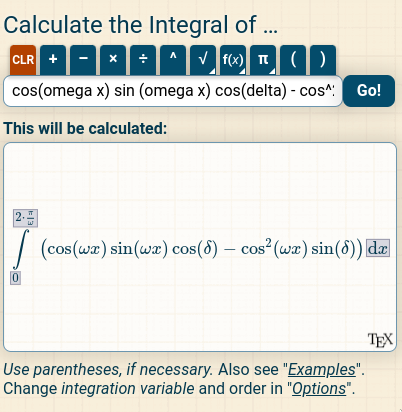
\includegraphics[width=0.4\textwidth]{ss/sshw4/kk1.png}
	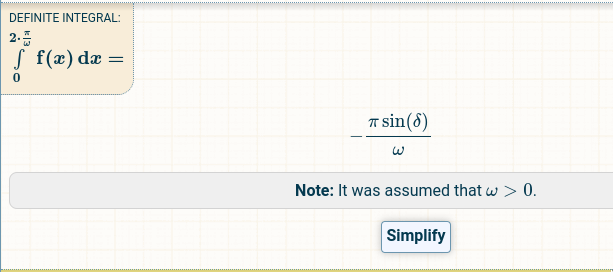
\includegraphics[width=0.4\textwidth]{ss/sshw4/kk2.png}
	\caption{ss/sshw4/kk2.png}
	\label{fig:ss-sshw4-kk2-png}
\end{figure}
Now, for $\tan \delta$ we can find $\sin \delta$ through 
\[
\sin \delta = \frac{2 \beta \omega}{\sqrt{(\omega_0 ^2 - \omega^2 )^2 + 4 \beta^2 \omega^2} }
\] 
Hence 
\[
W = - \pi CD \sin \delta  = \boxed{
- \pi C^2 \frac{2 \beta \omega }{(\omega_0 ^2 - \omega^2 )^2 + 4 \beta^2 \omega^2}
}\]

\subsection*{II}
\begin{align*}
	-W &= \int_{t_i}^{t_f}  F  v \, \mathrm{d} t \\ 
	&= \int_{t_i}^{t_f} -2 \beta v^2 \, \mathrm{d} t  \\
	W &= 2 \beta \int_{t_i}^{t_f} \omega^2 D^2 \sin ^2\left(\omega t - \delta\right) \, \mathrm{d} t   \\
	&= 2 \beta \omega^2 D^2 \frac{\pi}{\omega} \\
	&= \boxed{
	\pi C^2 \frac{2 \beta \omega}{\left(\omega_0^2 - \omega^2\right)^2 + 4 \beta^2 \omega^2} }\\
\end{align*}

\subsection*{III} 
The work done by the drag force is exactly counter balanced with the work done by driving force. I was careful with magnitude and in each case I measured ,,Work done by - force" instead of ,,work done on - system". 
\[
	W_{\text{drag}} = - W_{\text{driven}}
\] 

\subsection*{IV} 
The mass doesn't matter because we picked $C$ to be arbitrary, hence we can make our lives easier by just considering $m = 1$. 
\begin{align*}
	E = \frac{1}{2} v^2 + \frac{1}{2} kx ^2 &= 
\frac{1}{2} v^2 + \frac{1}{2} \omega_0^2 x ^2 
	\\
&=  \frac{1}{2} \dot{x	}(t)^2 + \frac{1}{2} \omega_0^2 x(t) ^2 
	\\
	\langle E \rangle = 
	\frac{\int_{t_i}^{t_f} E \, \mathrm{d} t }{\int_{t_i}^{t_f} \mathrm{d} t } &= 
\frac{1}{2 }\frac{1}{t_f - t_i} \left(
	\int_{t_i}^{t_f} \dot{x}(t)^2 \, \mathrm{d} t + 
	\omega_0^2 \int_{t_i}^{t_f} x(t)^2  \, \mathrm{d} t
\right)
	\\ 
	&= 
\frac{1}{2} \left(\frac{\omega}{2 \pi }\right) 
\left( \omega^2 D^2 
\int_{t_i}^{t_f} \sin^2(\omega t - \delta ) \, \mathrm{d} t   
+ 
\omega_0^2  D^2
\int_{t_i}^{t_f}   \cos ^2 (\omega t - \delta) \, \mathrm{d}  t
\right)
	\\
	&= 
\frac{1}{2} \left(\frac{\omega}{2 \pi }\right) 
\left( \omega^2 D^2 
	\left( \frac{\pi}{\omega }\right)+ 
\omega_0^2  D^2
\left(\frac{\pi}{\omega}\right)\right)
	\\
	&= 
\frac{1}{4} D^2 \left(\omega^2 + \omega_0^2\right)
	\\
	&= \boxed{
\frac{C^2}{4} \frac{\left(\omega_0^2 + \omega^2 \right)}{\left(\omega_0^2 - \omega ^2\right)^2 + 4 \beta ^2 \omega^2}
}	\\
\end{align*}

\subsection*{V}
\begin{align*}
	\frac{\text{Energy Lost}}{\text{Energy stored}} &= 
\pi C^2 \frac{2 \beta \omega}{ \mathcal Z} \cdot \frac{4}{C^2} \frac{\mathcal Z}{\omega_0^2 + \omega^2 }
	\\
	&=\boxed{
8 \pi \frac{\omega \beta}{\omega_0^2 + \omega^2}
}	\\
&\approx
8 \pi \frac{\omega_0 \beta}{2 \omega_0^2} \tag{$\beta \to 0 \implies \omega_0 \approx \omega$}
\\
&= 
4\pi \frac{\beta}{\omega_0}
\\
&= 
2\pi \left(\frac{2 \beta}{\omega_0}\right)
\\
&= \boxed{
\frac{2\pi}{Q}
}\\
\end{align*}

\section*{Problem 02}
\begin{align*}
x(t)	&=  D \cos \left( \omega t - \delta \right)\\
v(t) &= - \omega D \sin( \omega t - \delta ) \\
v^2(t) &= \omega^2 D^2 \sin ^2 \left( \omega t - \delta \right) \\
\langle v^2 (t) \rangle &= \frac{1}{2 } \omega ^2 D ^2  \\
\langle K \rangle &= \frac{m}{4} \omega^2 D^2 \\ 
&= \frac{m}{4} \omega ^2 C^2 \left(\frac{1}{- \omega^2 + 2 i \gamma \omega + \omega_0^2} \right) \left(\frac{1}{- \omega^2 - 2 i \gamma \omega + \omega_0^2}\right)\\
&= \boxed{
 \frac{m}{4} \left(\frac{\omega ^2 C^2 }{(\omega_0^2 - \omega^2 )^2 + \left(2  \gamma \omega\right) ^2}\right) }\\
\end{align*}
For $\omega = n \omega_0$ 
\begin{align*}
	\langle K \rangle &= \frac{m}{4}
 \frac{n^2 \omega_0 ^2 C^2}{\omega_0^{4} \left(1 - n^2\right) ^2 + 4 \gamma^2 n^2 \omega_0 ^2}
	\\ &= \frac{m}{4} \frac{C^2}{\omega_0^2 \left(\frac{1 - n^2}{n}\right)^2 + 4 \gamma^2 } \\
\end{align*}

For one octave higher, 
\[
\frac{1 - n^2}{n} = \frac{1 - 2^2}{2} = \frac{1 - 4}{2} = - \frac{3}{2} 
\] 
For one octave lower, 
\[ \frac{1 - n^2}{n} = 
	\frac{1 - (1 / 2)^2 }{(1 / 2)} =  \frac{1 - \frac{1}{4}}{\frac{1}{2}} = \frac{\frac{3}{4}}{\frac{1}{2}} = \frac{3}{2} 
\]
\emph{Now my goal is to show that $k$-octave higher average kinetic energy $\langle K \rangle (2^{k} \omega_0 )$ is equal to $k$-octave lower $\langle K \rangle (2^{-k} \omega_0 ) $. Revising the later text it feels like a pure math proof that doesn't make sense in the first look.}


Let any higher octave be called $2^k = N$ and a lower octave by same distance be $2^{-k} = n$. Then it's obvious, 
\[ \frac{1- N^2}{N} =  
	\frac{1 - 2^{2k}}{2^k} = 2^{k} (2^{-k} - 2^k) \frac{1}{2^k} = \frac{1}{2^{-k}} (2^{-2k} - 1  ) = - \frac{1 - (2^{-k})^2}{2^{-k}}  = - \frac{1 - n^2}{n} 
\]{  
\[
\implies \left(\frac{1-N^2}{N}\right)^2 = \left( - \frac{1-n^2}{n}		\right)^2
\implies \langle K (\omega = 2^{k} \omega_0) \rangle  = 
\langle K( \omega = 2^{-k}\omega_0)  \rangle 
\]Hence we proved for two equally distant octaves the kinetic energy satisfies
\[
\boxed{
\langle K (2^{k} \omega_0) \rangle = 
\langle K (2^{-k} \omega_0) \rangle 
}
\] 

\newpage 
\section*{Problem 03}

For diagram purposes it's not a matter if we pick $m = 1$ to keep things simple. 
\[
U(x) = k \left(
- \frac{1}{2}x^2 + \frac{1}{4}\frac{x^4}{l^2}
\right)
\]
\begin{figure}[H]
	\centering
	\begin{tikzpicture}
		\begin{axis}[
			xmin= -5, xmax= 5,
			ymin= -5, ymax = 5,
			axis lines = middle,
		]
		\addplot[domain=-5:5, samples=100]{(1.5)*( -(x^2/2) + (x^4 / (4*(1.5)^2)) )};
		\end{axis}
	\end{tikzpicture}\hfill
	\begin{tikzpicture}
		\begin{axis}[
			xmin= -5, xmax= 5,
			ymin= -5, ymax = 5,
			axis lines = middle,
		]
		\addplot[domain=-5:5, samples=100]{(-1.5)*( -(x^2/2) + (x^4 / (4*(1.5)^2)) )};
		\end{axis}
	\end{tikzpicture}
	\caption{For the choice $(k,l) = (1.5, 1.5)$ and $(k,l) = (-1.5, 1.5)$}
	\label{}
\end{figure}
But we can directly find $v(x)$ dependence from this. Implying conservation of energy $E$, 
\begin{align*}
	E &= K(x ) + U(x) \\ 
E	&= \frac{1}{2} v^2(x) + U(x)  \\
E - U(x)	
	&=  \frac{1}{2}v^2(x)\\
2 ( E - U(x)) &= v^2(x)
\implies \sqrt{2 (E - U(x) ) } = v(x) = p(x)
\end{align*}
We can make plots for various values of $E$ which imply various starting energy. 


\begin{figure}[H]
	\centering
	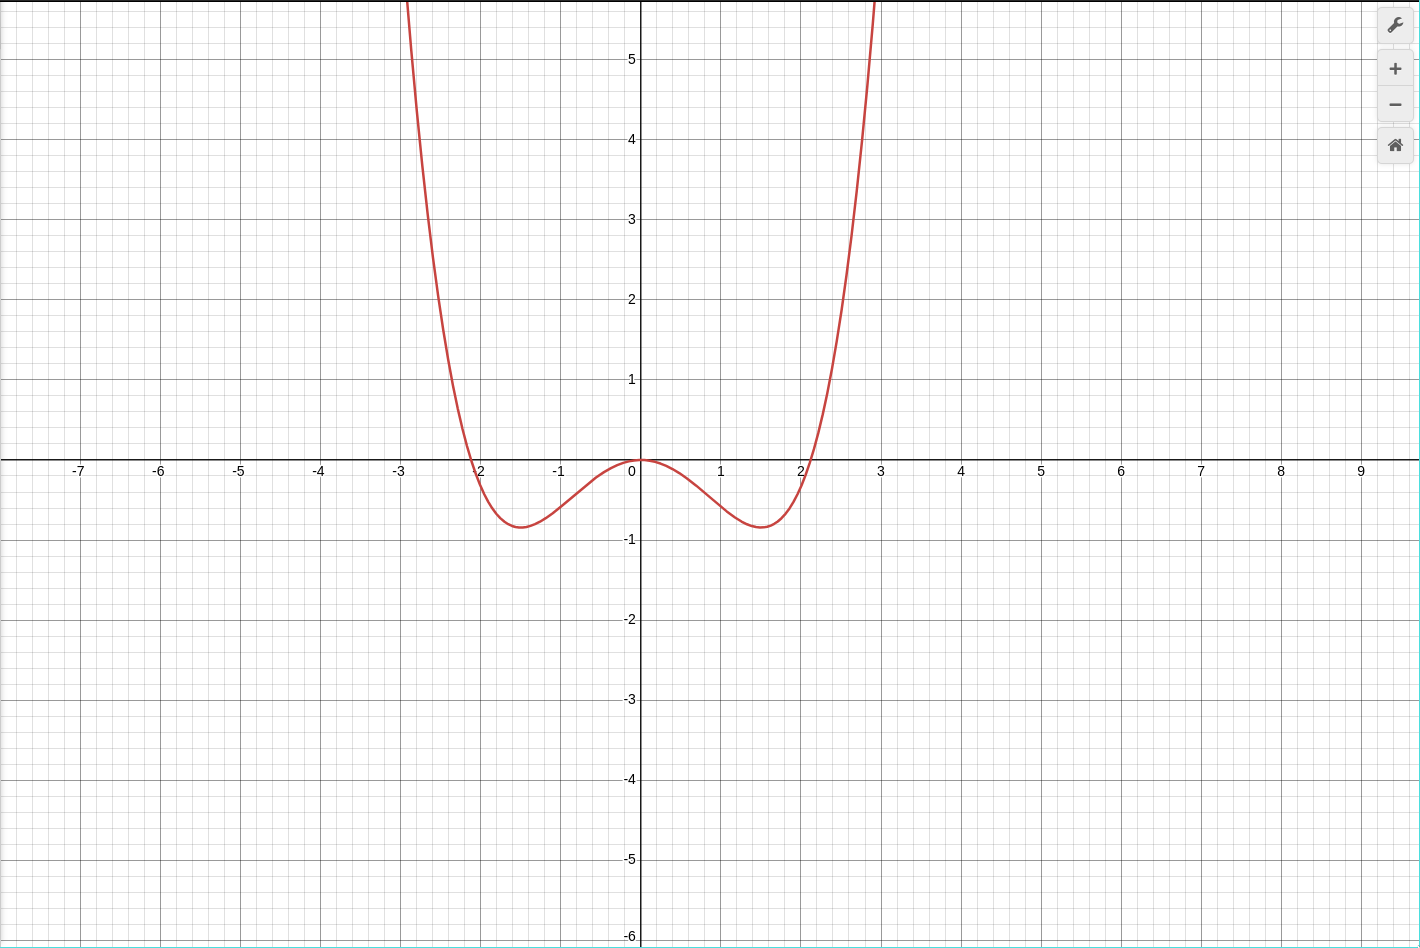
\includegraphics[width=0.4\textwidth]{ss/dsms01.png}
	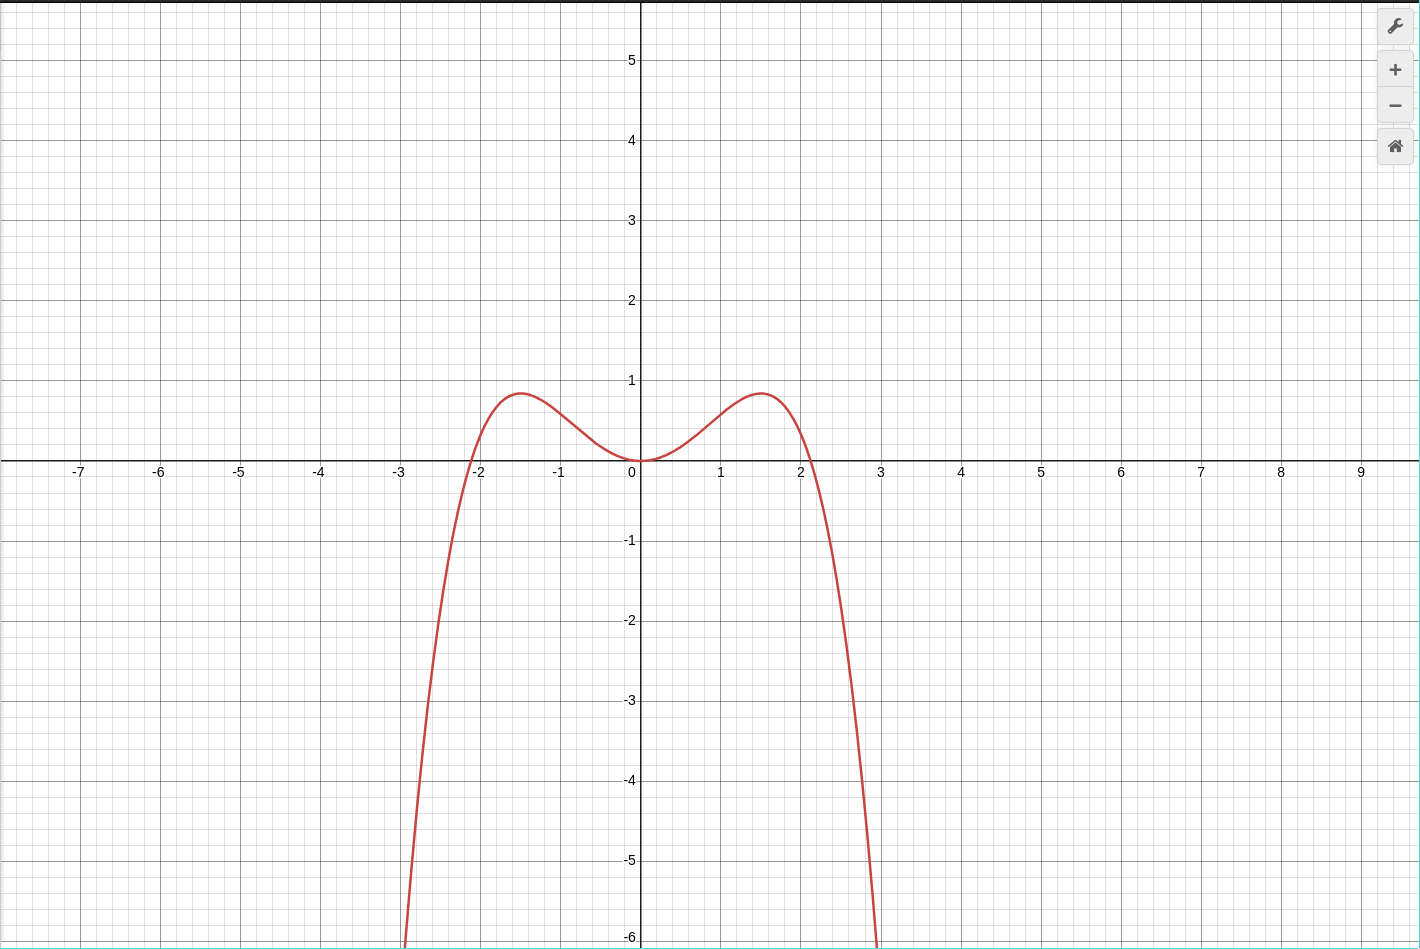
\includegraphics[width=0.4\textwidth]{ss/dsms4.png}
	\caption{A standard plot for the $U(x)$ where $(k,l) = (1.5,1.5)$ and $(-1.5,1.5)$}
	\label{fig:ss-dsms1-png}
\end{figure}
\newpage 
Now what I am going to do is plot $U(x)$ vs $x$ and also $p(x)$ vs $x$ on the same plot to AeStHeTicaLLy visualize the energy and phase diagram together. The purple/violet dotted lines represent the possible paths the particle might take given the initial conditions. 
\subsection*{$k>0$ }
\begin{figure}[H]
	\centering
	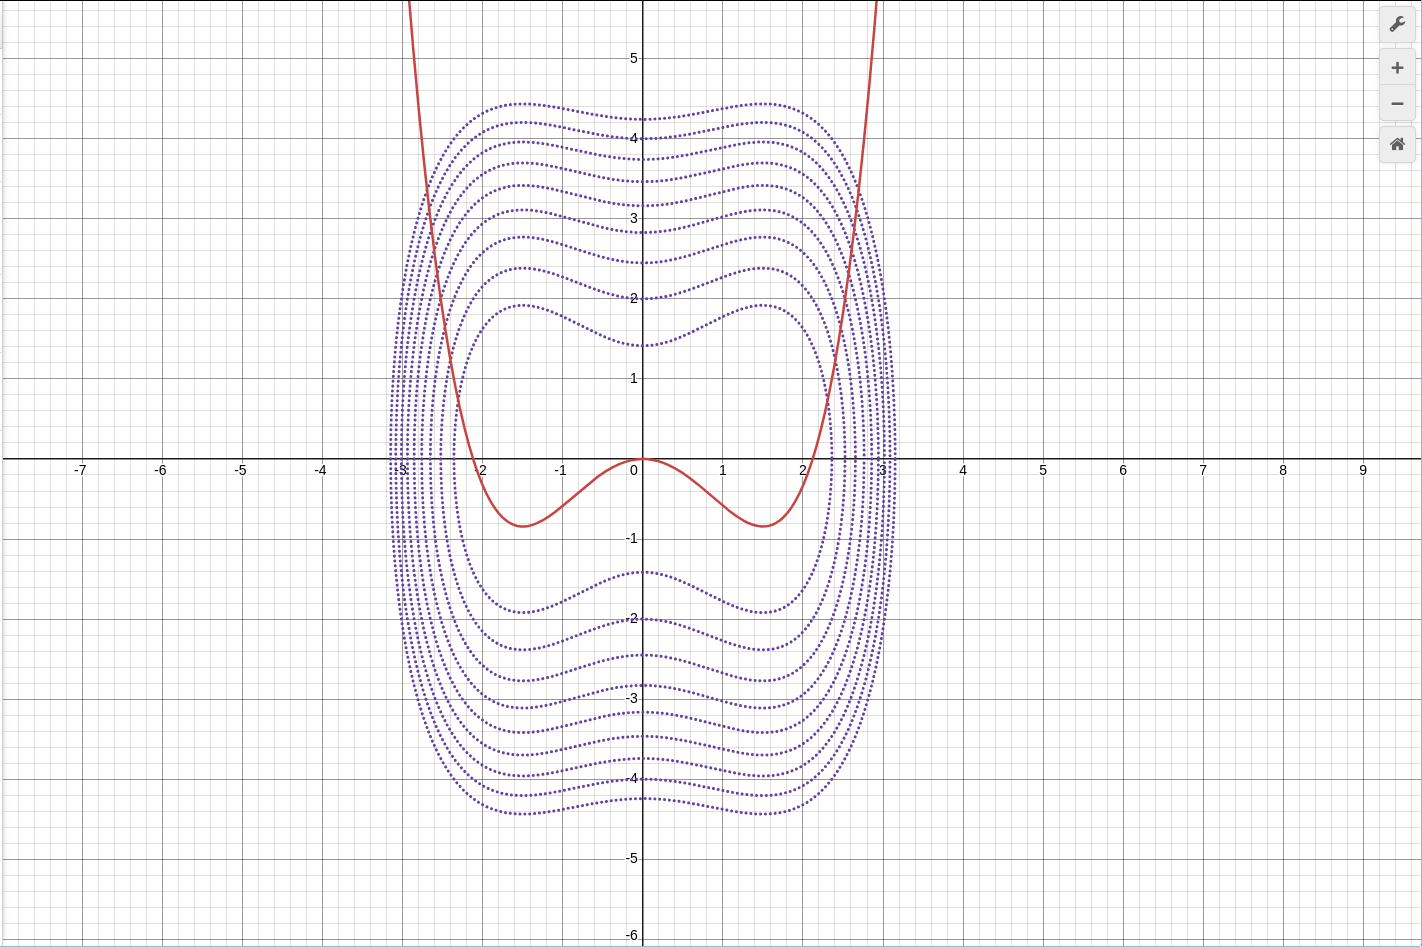
\includegraphics[width=0.9\textwidth]{ss/dsms2.png}
	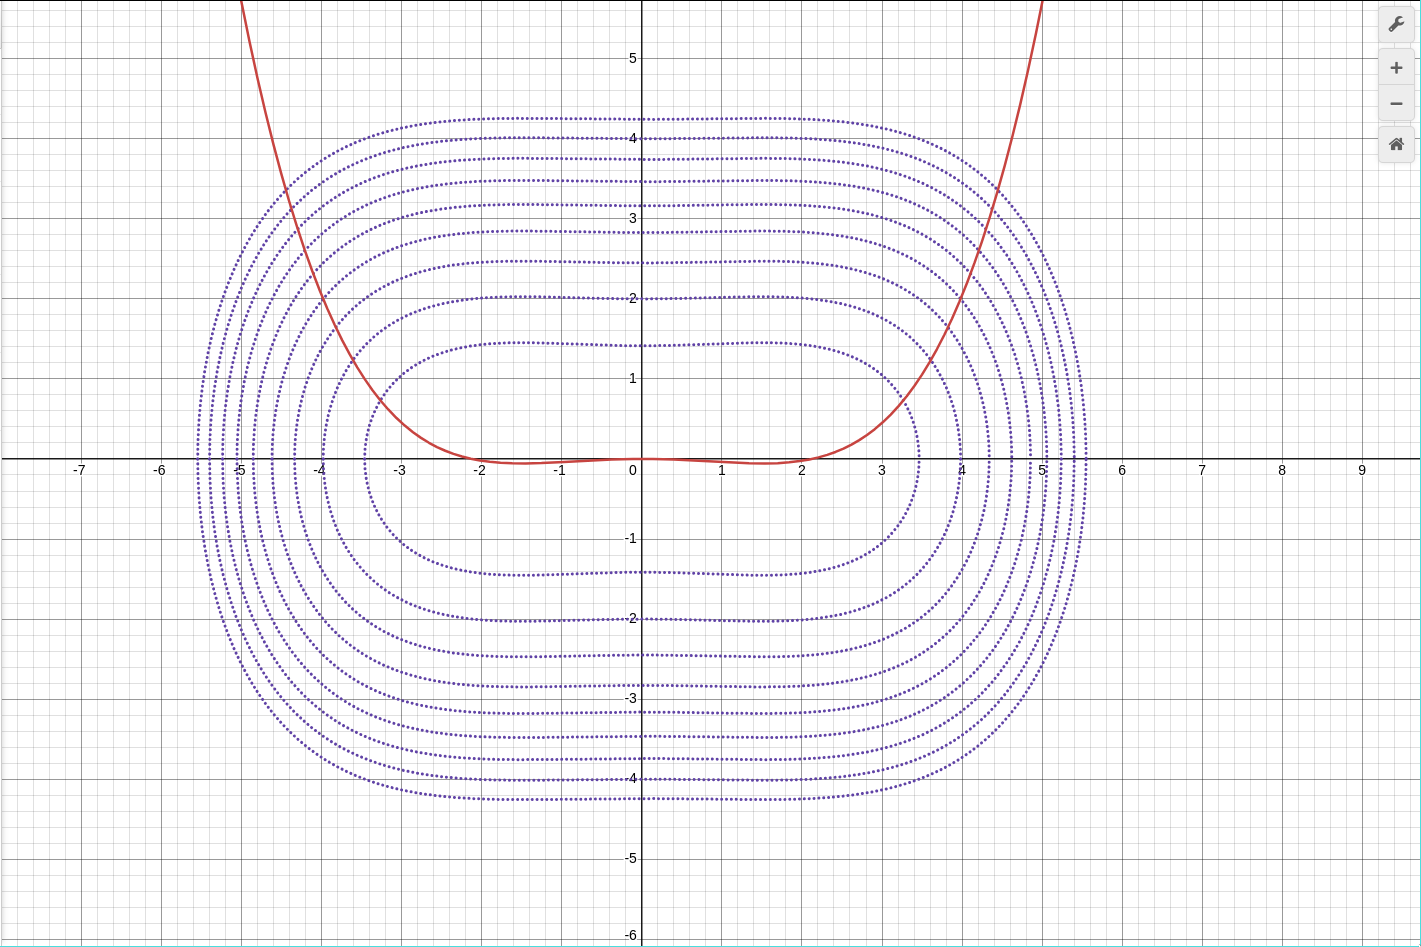
\includegraphics[width=0.9\textwidth]{ss/dsms3.png}
	\caption{$(k,l) = (1.5,1.5)$ and $(k,l) = (0.1,1.5)$ where total energy $E = \{1,2, \ldots, 9\} $}
	\label{fig:ss-dsms3-png}
\end{figure}

\subsection*{$k<0$ }
\begin{figure}[H]
	\centering
	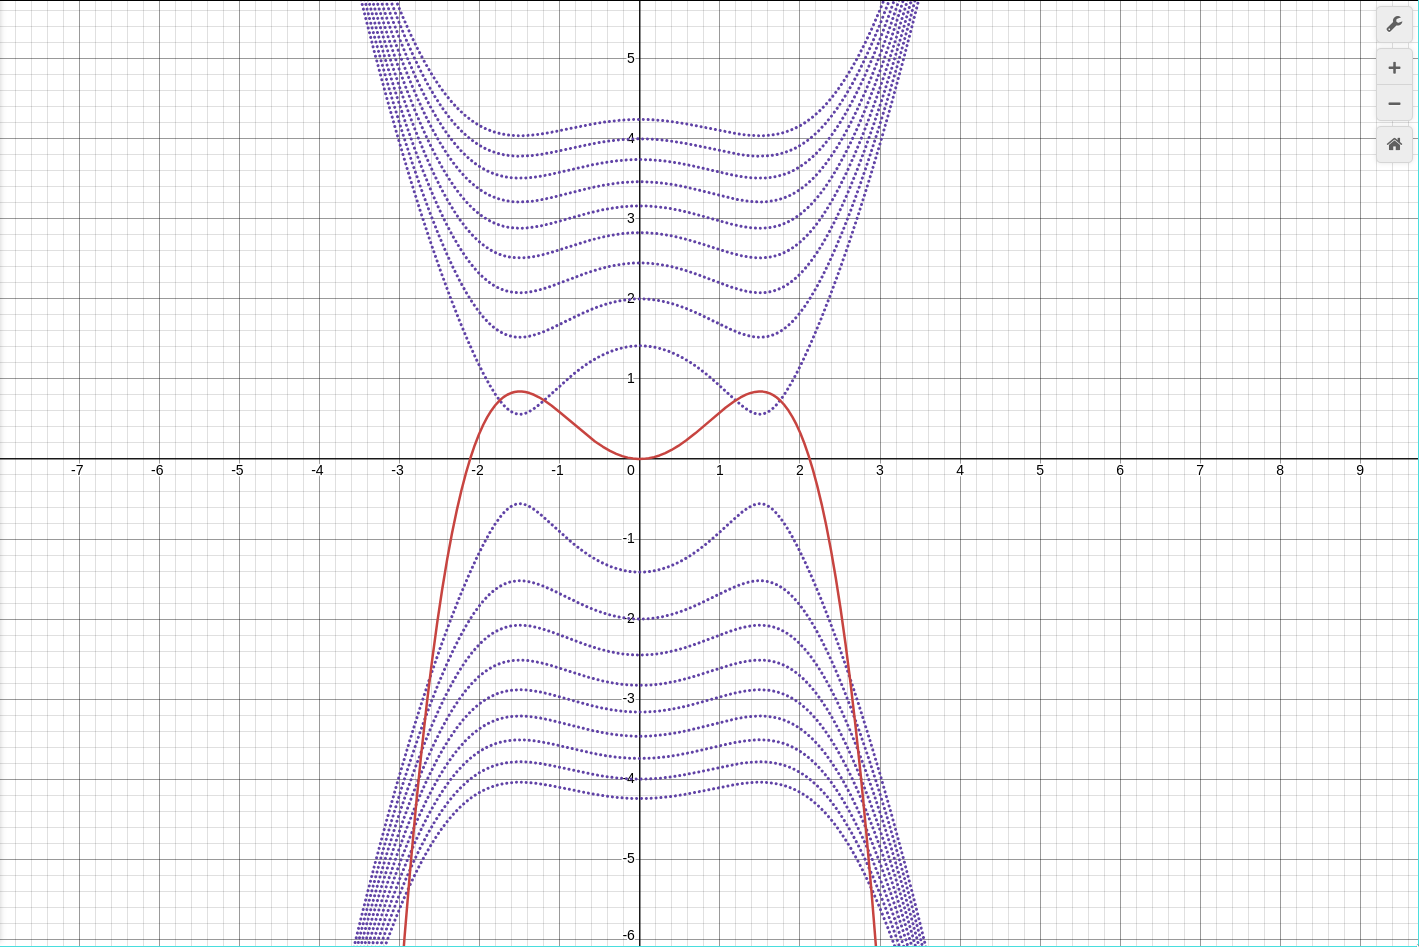
\includegraphics[width=0.9\textwidth]{ss/dsmsN1.png}
	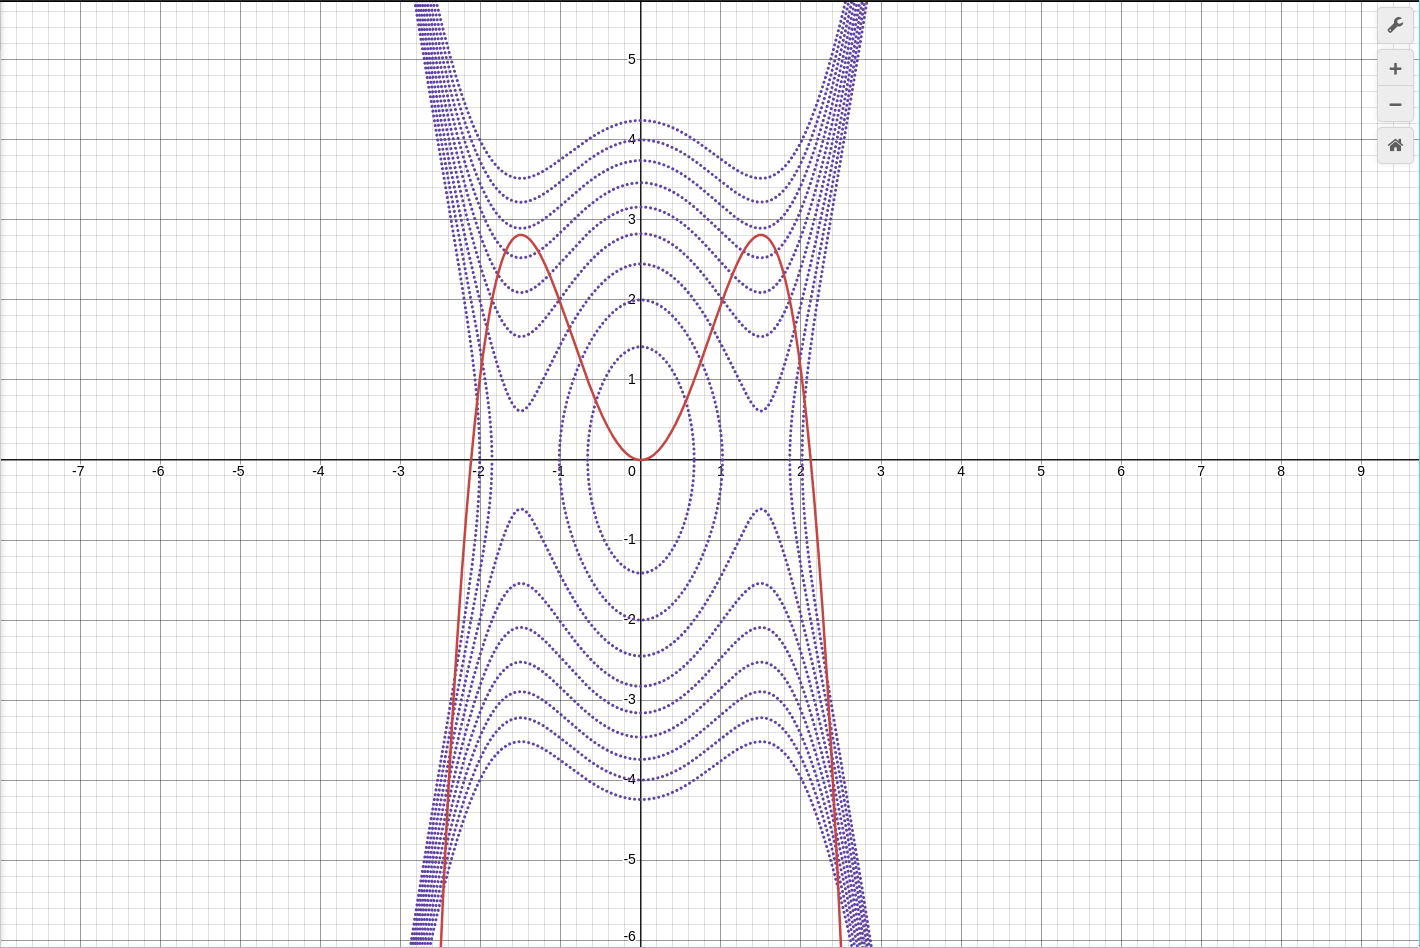
\includegraphics[width=0.9\textwidth]{ss/dsmsN2.png}
	\caption{Same energy(s) and $(k,l) = (-1.5,1.5), (-5,1.5)$}
	\label{fig:ss-dsmsN2-png}
\end{figure}



\begin{figure}[H]
	\centering
	\frame{ 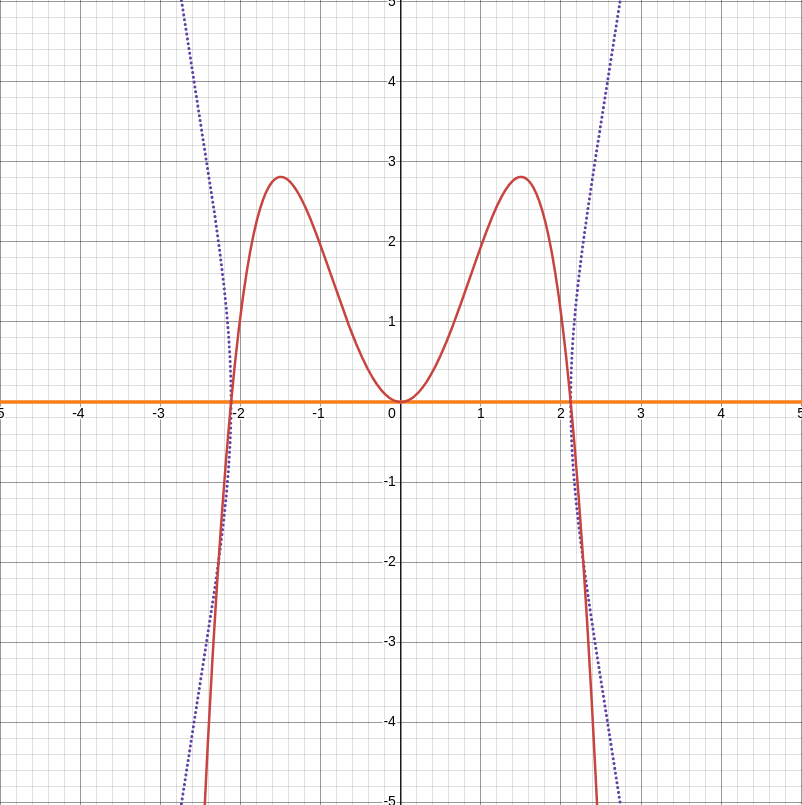
\includegraphics[width=0.3\textwidth]{ss/opc1.png}}
	\frame{ 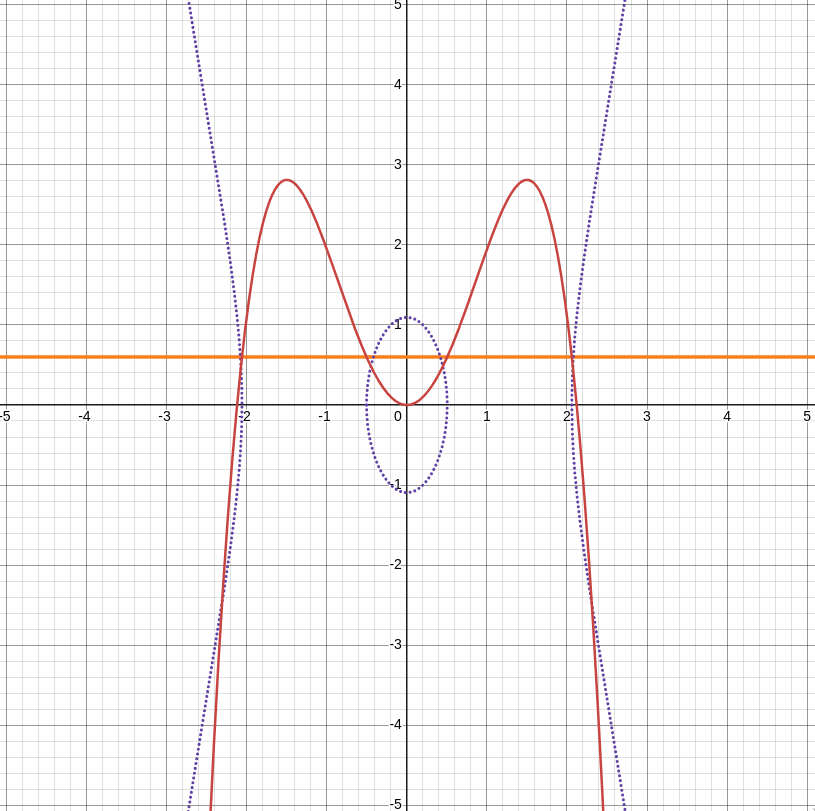
\includegraphics[width=0.3\textwidth]{ss/opc2.png}}
	\frame{	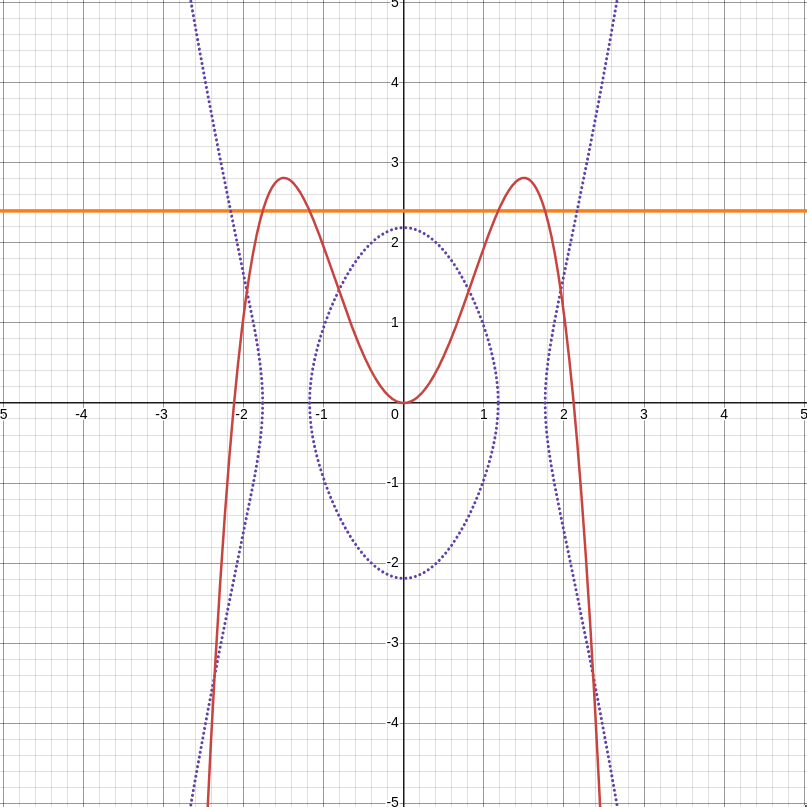
\includegraphics[width=0.3\textwidth]{ss/opc3.png}}
	\frame{	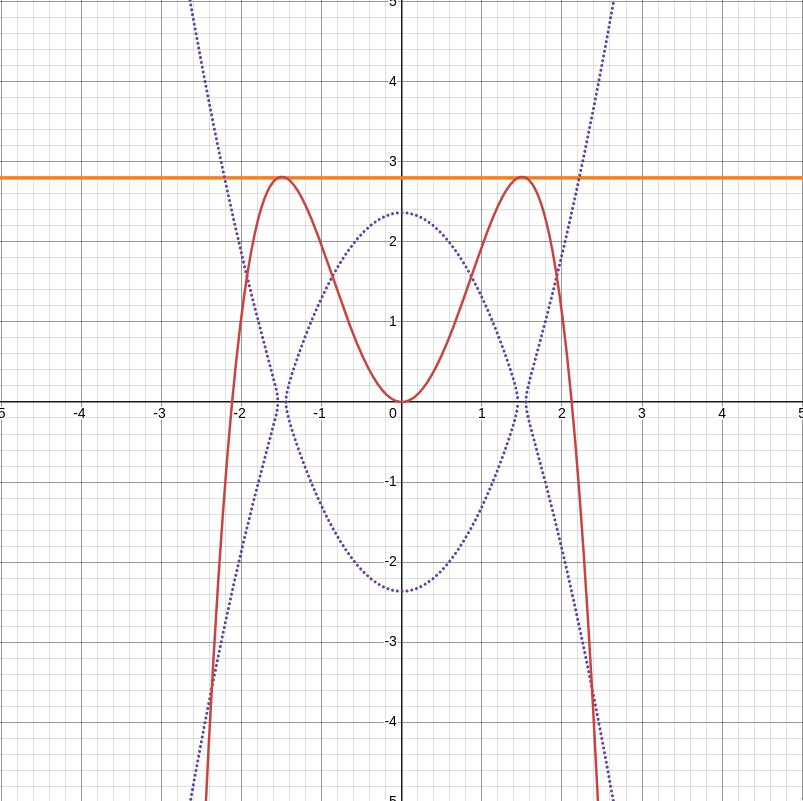
\includegraphics[width=0.3\textwidth]{ss/opc4.png}}
	\frame{	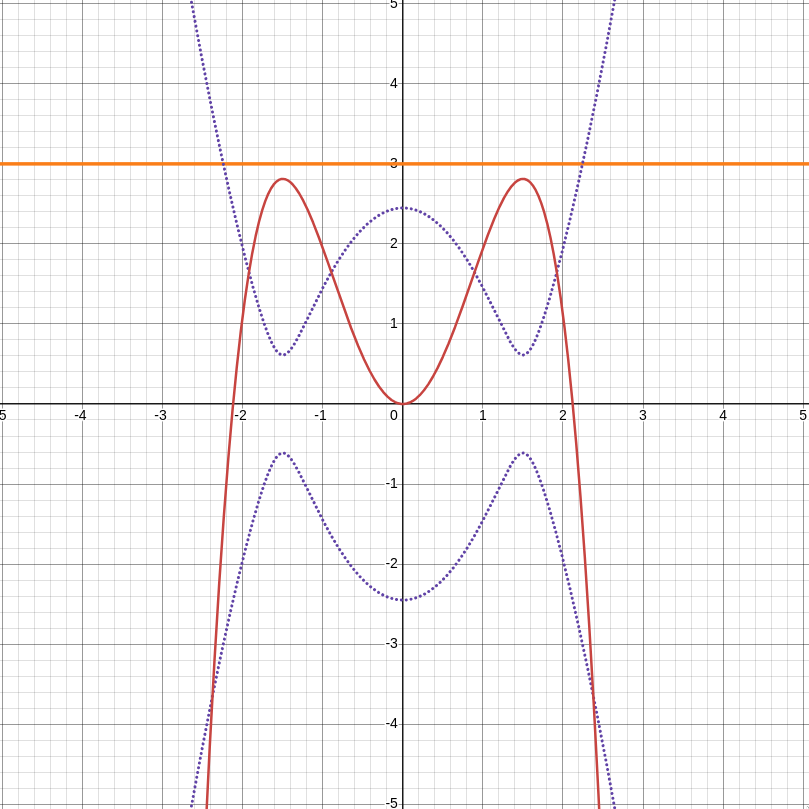
\includegraphics[width=0.3\textwidth]{ss/opc5.png}}
	\frame{	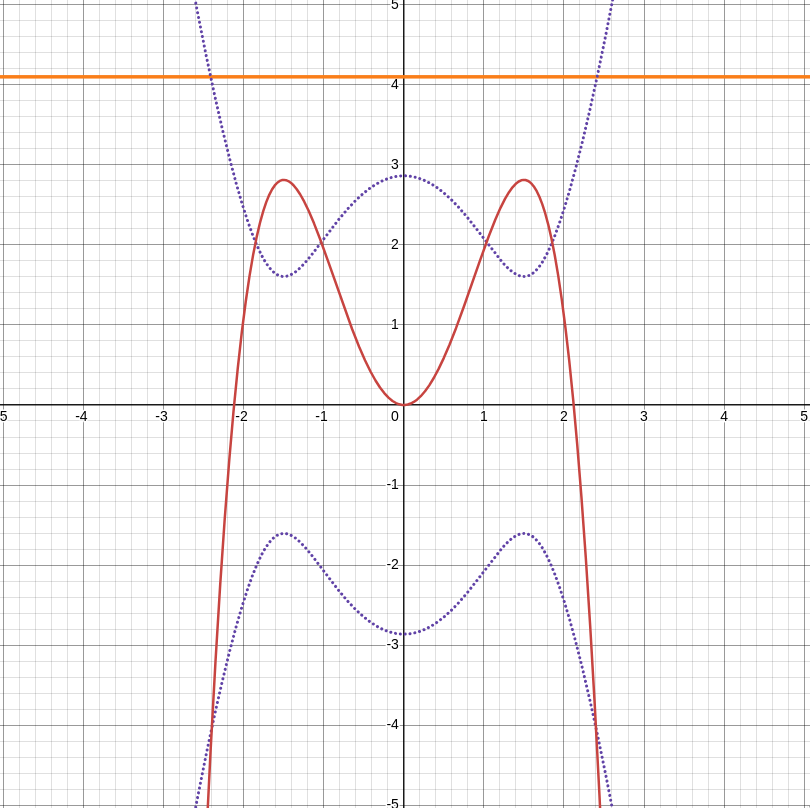
\includegraphics[width=0.3\textwidth]{ss/opc6.png}}
	\caption{ss/opc6.png}
	\label{fig:ss-opc6-png-}
\end{figure}
\textbf{Description:} Every closed loop means the particle is trapped in the well. This closed loop for one-dimensional case implies the particle goes back and forth. In the 6 tiles of diagrams above I also plotted the total energy as a horizontal bar. For the total energy $E$ lower than the peak of $U(x)$, we see that the particle is usually trapped in a loop in phase diagram. Just the moment the $E$ bar goes over the peak of $U(x)$, the particle is free and the loop of phase diagram breaks. The particle has escaped the well. 

It's impossible for the particle to escape $k>0$ cases because the well is infinite. $k<0$ is possible to leave for energies above a limit but if the particle escapes, it achieves infinite speed as it keeps accelerating given $U(x)$ extends to negative infinity. 
\newpage
\section*{Problem 04} 
\[
\ddot{x} + \beta(\dot{x}^2) \text{ Sign}(\dot{x})  + x = F_0 \cos(\omega_D t)
\]

\subsection*{Plots for $\beta = 0.1$ and $\omega_D = \{0.3, 3\} $}
\begin{tcolorbox}[sharpish corners]
	\begin{figure}[H]
		\centering
		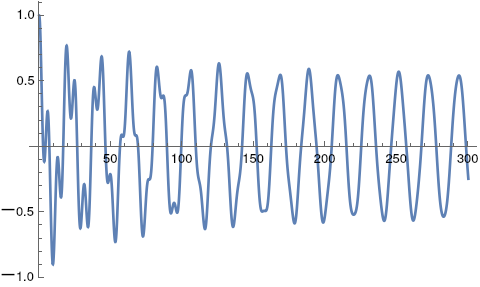
\includegraphics[width=0.6\textwidth]{ss/lst03.png}
		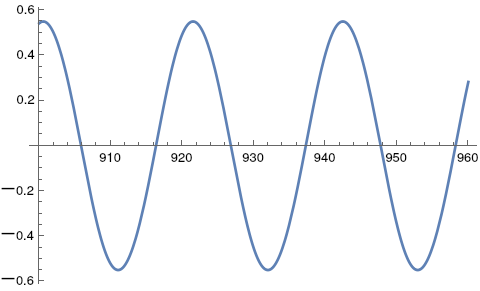
\includegraphics[width=0.6\textwidth]{ss/honky2.png}
		\caption{ss/lst1.png}
		\label{fig:ss-lst1-png}
	\end{figure}
\begin{lstlisting}[language=Mathematica]
b = 0.1
F0 = 0.5
w = 0.3
P = NDSolve[{x''[t] + Sign[x'[t]]*b*(x'[t])^2 + x[t] == F0*Cos[w*t], 
    x[0] == 1, x'[0] == 0}, x, {t, 0, 1000}];
Plot[Evaluate[x[t] /. P], {t, 0, 300}, PlotRange -> All]\end{lstlisting}
\end{tcolorbox}

\begin{tcolorbox}[sharpish corners]
	\begin{figure}[H]
		\centering
		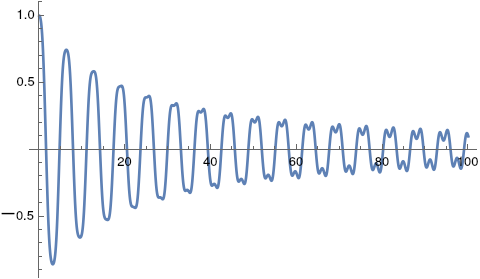
\includegraphics[width=0.6\textwidth]{ss/lst04.png}
		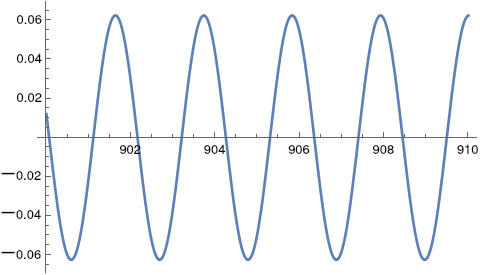
\includegraphics[width=0.6\textwidth]{ss/honky1.png}
		\caption{ss/lst1.png}
		\label{fig:ss-lst1-png}
	\end{figure}
\begin{lstlisting}[language=Mathematica]
b = 0.1
F0 = 0.5
w = 3
P = NDSolve[{x''[t] + Sign[x'[t]]*b*(x'[t])^2 + x[t] == F0*Cos[w*t], 
    x[0] == 1, x'[0] == 0}, x, {t, 0, 1000}];
Plot[Evaluate[x[t] /. P], {t, 0, 100}, PlotRange -> All]
\end{lstlisting}
\end{tcolorbox}





\subsection*{Plots for $\beta = 0.3$ and $\omega_D = \{0.3, 3\} $}
\begin{tcolorbox}[sharpish corners]
	\begin{figure}[H]
		\centering
		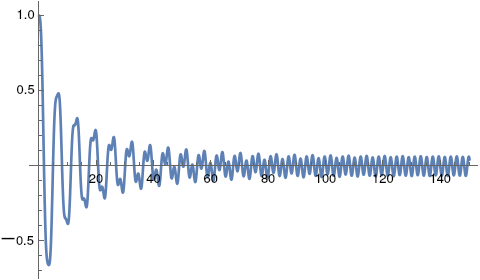
\includegraphics[width=0.6\textwidth]{ss/lst1.png}
		\caption{ss/lst1.png}
		\label{fig:ss-lst1-png}
	\end{figure}
\begin{lstlisting}[language=Mathematica]
b = 0.3
F0 = 0.5
w = 3
P = NDSolve[
	{x''[t] + Sign[x'[t]]*b*(x'[t])^2 + x[t] == F0*Cos[w*t], 
    	x[0] == 1, x'[0] == 0}, 
    	x, {t, 0, 1000}];
Plot[Evaluate[x[t] /. P], {t, 0, 150}, PlotRange -> All]
\end{lstlisting}
\end{tcolorbox}


\begin{tcolorbox}[sharpish corners]
	\begin{figure}[H]
		\centering
		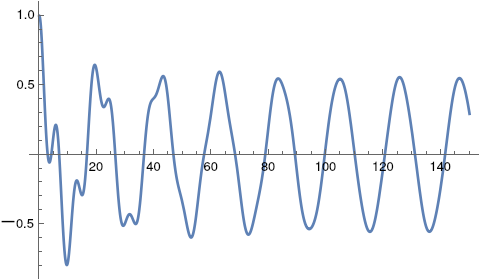
\includegraphics[width=0.6\textwidth]{ss/lst02.png}
		\caption{ss/lst1.png}
		\label{fig:ss-lst1-png}
	\end{figure}
\begin{lstlisting}[language=Mathematica]
b = 0.3
F0 = 0.5
w = 0.3
P = NDSolve[{x''[t] + Sign[x'[t]]*b*(x'[t])^2 + x[t] == F0*Cos[w*t], 
    x[0] == 1, x'[0] == 0}, x, {t, 0, 1000}];
Plot[Evaluate[x[t] /. P], {t, 0, 150}, PlotRange -> All]
\end{lstlisting}
\end{tcolorbox}



\subsection*{Plots for $\beta = 1$ and $\omega_D = \{0.3, 3\} $ }
\begin{tcolorbox}[sharpish corners]
	\begin{figure}[H]
		\centering
		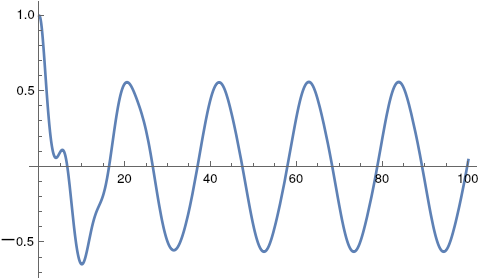
\includegraphics[width=0.6\textwidth]{ss/honky3.png}
		\caption{ss/lst1.png}
		\label{fig:ss-lst1-png}
	\end{figure}
\begin{lstlisting}[language=Mathematica]
b = 1
F0 = 0.5
w = 0.3
P = NDSolve[{x''[t] + Sign[x'[t]]*b*(x'[t])^2 + x[t] == F0*Cos[w*t], 
    x[0] == 1, x'[0] == 0}, x, {t, 0, 1000}];
Plot[Evaluate[x[t] /. P], {t, 0, 100}, PlotRange -> All] 
\end{lstlisting}
\end{tcolorbox}


\begin{tcolorbox}[sharpish corners]
	\begin{figure}[H]
		\centering
		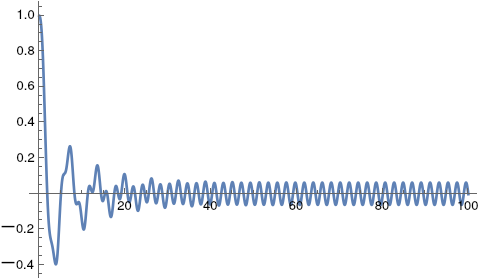
\includegraphics[width=0.6\textwidth]{ss/honky4.png}
		\caption{ss/lst1.png}
		\label{fig:ss-lst1-png}
	\end{figure}
\begin{lstlisting}[language=Mathematica]
b = 1
F0 = 0.5
w = 3
P = NDSolve[{x''[t] + Sign[x'[t]]*b*(x'[t])^2 + x[t] == F0*Cos[w*t], 
    x[0] == 1, x'[0] == 0}, x, {t, 0, 1000}];
Plot[Evaluate[x[t] /. P], {t, 0, 100}, PlotRange -> All] 
\end{lstlisting}
\end{tcolorbox}

\newpage
\subsection*{Plots for $\beta = 3$ and $\omega_D = \{0.3, 3\} $ }

\begin{tcolorbox}[sharpish corners]
	\begin{figure}[H]
		\centering
		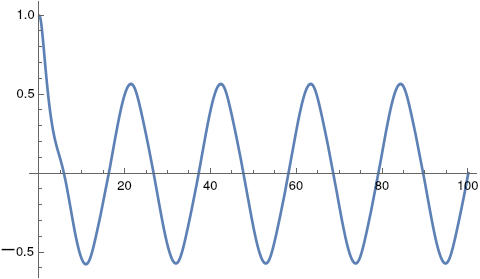
\includegraphics[width=0.6\textwidth]{ss/honky5.png}
		\caption{ss/lst1.png}
		\label{fig:ss-lst1-png}
	\end{figure}
\begin{lstlisting}[language=Mathematica]
b = 3
F0 = 0.5
w = 0.3
P = NDSolve[{x''[t] + Sign[x'[t]]*b*(x'[t])^2 + x[t] == F0*Cos[w*t], 
    x[0] == 1, x'[0] == 0}, x, {t, 0, 1000}];
Plot[Evaluate[x[t] /. P], {t, 0, 100}, PlotRange -> All] 
\end{lstlisting}
\end{tcolorbox}



\begin{tcolorbox}[sharpish corners]
	\begin{figure}[H]
		\centering
	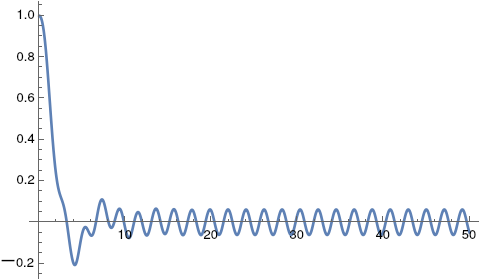
\includegraphics[width=0.6\textwidth]{ss/honky6.png}
		\caption{ss/lst1.png}
		\label{fig:ss-lst1-png}
	\end{figure}
\begin{lstlisting}[language=Mathematica]
b = 3
F0 = 0.5
w = 3
P = NDSolve[{x''[t] + Sign[x'[t]]*b*(x'[t])^2 + x[t] == F0*Cos[w*t], 
    x[0] == 1, x'[0] == 0}, x, {t, 0, 1000}];
Plot[Evaluate[x[t] /. P], {t, 0, 50}, PlotRange -> All]
\end{lstlisting}
\end{tcolorbox}

\newpage
\subsection*{Linear Dampening Case} 
\[
\ddot{x} + \beta \dot{x} + x = F_0 \cos(\omega_D t) \]

\subsection{For $\omega_D = 3$ and $\beta = \{0.1,0.3,1,3\}$ }
\begin{tcolorbox}[sharpish corners]
	\begin{figure}[H]
		\centering
		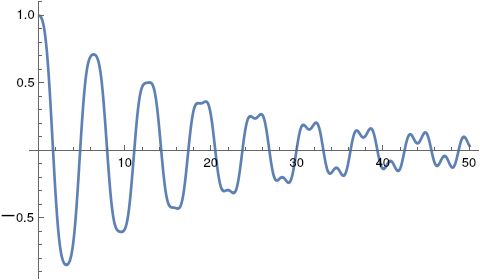
\includegraphics[width=0.6\textwidth]{ss/sshw4/1.png}
		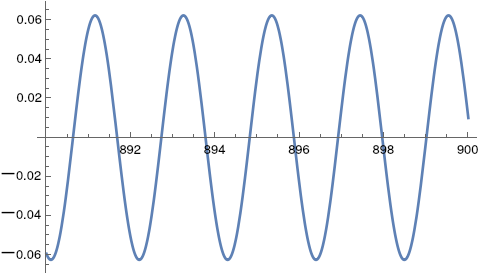
\includegraphics[width=0.6\textwidth]{ss/sshw4/11.png}
		\caption{ss/lst1.png}
		\label{fig:ss-lst1-png}
	\end{figure}
\begin{lstlisting}[language=Mathematica]
b = 0.1
F0 = 0.5
w = 3
P = NDSolve[{x''[t] + b*(x'[t]) + x[t] == F0*Cos[w*t], x[0] == 1, 
    x'[0] == 0}, x, {t, 0, 1000}];
Plot[Evaluate[x[t] /. P], {t, 0, 50}, PlotRange -> All]
\end{lstlisting}
\end{tcolorbox}

\begin{tcolorbox}[sharpish corners]
	\begin{figure}[H]
		\centering
		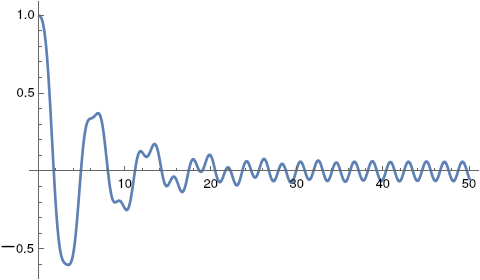
\includegraphics[width=0.6\textwidth]{ss/sshw4/2.png}
		\caption{ss/lst1.png}
		\label{fig:ss-lst1-png}
	\end{figure}
\begin{lstlisting}[language=Mathematica]
b = 0.3
F0 = 0.5
w = 3
P = NDSolve[{x''[t] + b*(x'[t]) + x[t] == F0*Cos[w*t], x[0] == 1, 
    x'[0] == 0}, x, {t, 0, 1000}];
Plot[Evaluate[x[t] /. P], {t, 0, 50}, PlotRange -> All]
\end{lstlisting}
\end{tcolorbox}

\begin{tcolorbox}[sharpish corners]
	\begin{figure}[H]
		\centering
		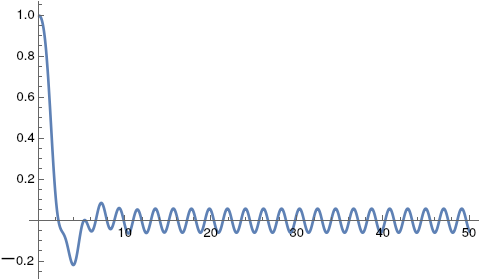
\includegraphics[width=0.6\textwidth]{ss/sshw4/3.png}
		\caption{ss/lst1.png}
		\label{fig:ss-lst1-png}
	\end{figure}
\begin{lstlisting}[language=Mathematica]
b = 1
F0 = 0.5
w = 3
P = NDSolve[{x''[t] + b*(x'[t]) + x[t] == F0*Cos[w*t], x[0] == 1, 
    x'[0] == 0}, x, {t, 0, 1000}];
Plot[Evaluate[x[t] /. P], {t, 0, 50}, PlotRange -> All]
\end{lstlisting}
\end{tcolorbox}

\begin{tcolorbox}[sharpish corners]
	\begin{figure}[H]
		\centering
		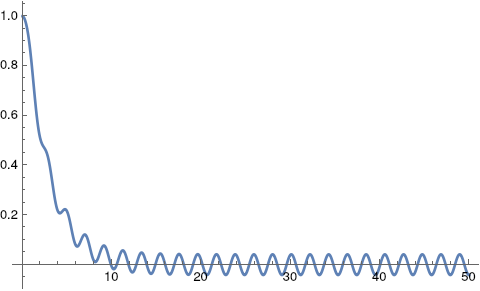
\includegraphics[width=0.6\textwidth]{ss/sshw4/4.png}
		\caption{ss/lst1.png}
		\label{fig:ss-lst1-png}
	\end{figure}
\begin{lstlisting}[language=Mathematica]
b = 3
F0 = 0.5
w = 3
P = NDSolve[{x''[t] + b*(x'[t]) + x[t] == F0*Cos[w*t], x[0] == 1, 
    x'[0] == 0}, x, {t, 0, 1000}];
Plot[Evaluate[x[t] /. P], {t, 0, 50}, PlotRange -> All]
\end{lstlisting}
\end{tcolorbox}


\newpage
\subsection{For $\omega_D = 0.3$ and $\beta = \{0.1,0.3,1,3\}$}
\begin{tcolorbox}[sharpish corners]
	\begin{figure}[H]
		\centering
		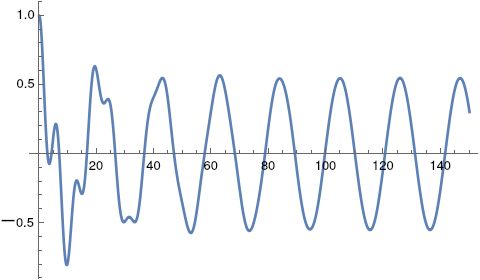
\includegraphics[width=0.6\textwidth]{ss/sshw4/5.png}
		\caption{ss/lst1.png}
		\label{fig:ss-lst1-png}
	\end{figure}
\begin{lstlisting}[language=Mathematica]
b = 0.1
F0 = 0.5
w = 0.3
P = NDSolve[{x''[t] + b*(x'[t]) + x[t] == F0*Cos[w*t], x[0] == 1, ]
    x'[0] == 0}, x, {t, 0, 1000}];
Plot[Evaluate[x[t] /. P], {t, 0, 150}, PlotRange -> All]
\end{lstlisting}
\end{tcolorbox}


\begin{tcolorbox}[sharpish corners]
	\begin{figure}[H]
		\centering
		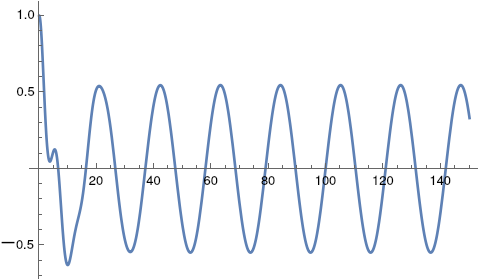
\includegraphics[width=0.6\textwidth]{ss/sshw4/6.png}
		\caption{ss/lst1.png}
		\label{fig:ss-lst1-png}
	\end{figure}
\begin{lstlisting}[language=Mathematica]
b = 0.3
F0 = 0.5
w = 0.3
P = NDSolve[{x''[t] + b*(x'[t]) + x[t] == F0*Cos[w*t], x[0] == 1, 
    x'[0] == 0}, x, {t, 0, 1000}];
Plot[Evaluate[x[t] /. P], {t, 0, 150}, PlotRange -> All]
\end{lstlisting}
\end{tcolorbox}

\begin{tcolorbox}[sharpish corners]
	\begin{figure}[H]
		\centering
		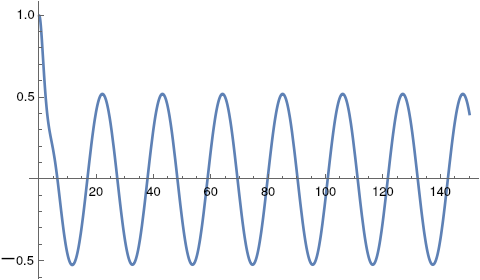
\includegraphics[width=0.6\textwidth]{ss/sshw4/7.png}
		\caption{ss/lst1.png}
		\label{fig:ss-lst1-png}
	\end{figure}
\begin{lstlisting}[language=Mathematica]
b = 1
F0 = 0.5
w = 0.3
P = NDSolve[{x''[t] + b*(x'[t]) + x[t] == F0*Cos[w*t], x[0] == 1, 
    x'[0] == 0}, x, {t, 0, 1000}];
Plot[Evaluate[x[t] /. P], {t, 0, 150}, PlotRange -> All]
\end{lstlisting}
\end{tcolorbox}

\begin{tcolorbox}[sharpish corners]
	\begin{figure}[H]
		\centering
		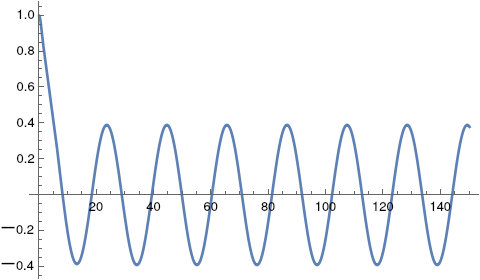
\includegraphics[width=0.6\textwidth]{ss/sshw4/8.png}
		\caption{ss/lst1.png}
		\label{fig:ss-lst1-png}
	\end{figure}
\begin{lstlisting}[language=Mathematica]
b = 3
F0 = 0.5
w = 0.3
P = NDSolve[{x''[t] + b*(x'[t]) + x[t] == F0*Cos[w*t], x[0] == 1, 
    x'[0] == 0}, x, {t, 0, 1000}];
Plot[Evaluate[x[t] /. P], {t, 0, 150}, PlotRange -> All]
\end{lstlisting}
\end{tcolorbox}

\textbf{Analysis: } From looking at the plots, we can roughly see that quadratic damping is very high compared to linear damping, but as oscillation amplitude gets smaller, quadratic damping gets even more lighter and oscillation reaches steady state. Qualitatively, for linear case it is more spread out. 

For Quadratic case it takes comparatively shorter time to reach steady state because of high damping. 
\newpage
\subsection*{b} 
Look, I can't use merely the above plots for finding another plot for $\omega_D$ versus the amplitude of steady state. There aren't enough $\omega_D$, just $0.3$ and $3$. I will do the plot from scratch. 

We look at the data from the plot. There are too many choices for $\beta$ so we will just go with $\beta = 1$. 

\[
\ddot{x} + (1) \text{Sign}(\dot{x})(\dot{x})^2  + \omega  = (0.5) \cos(\omega_D t)
\]
\begin{figure}[H]
	\centering
	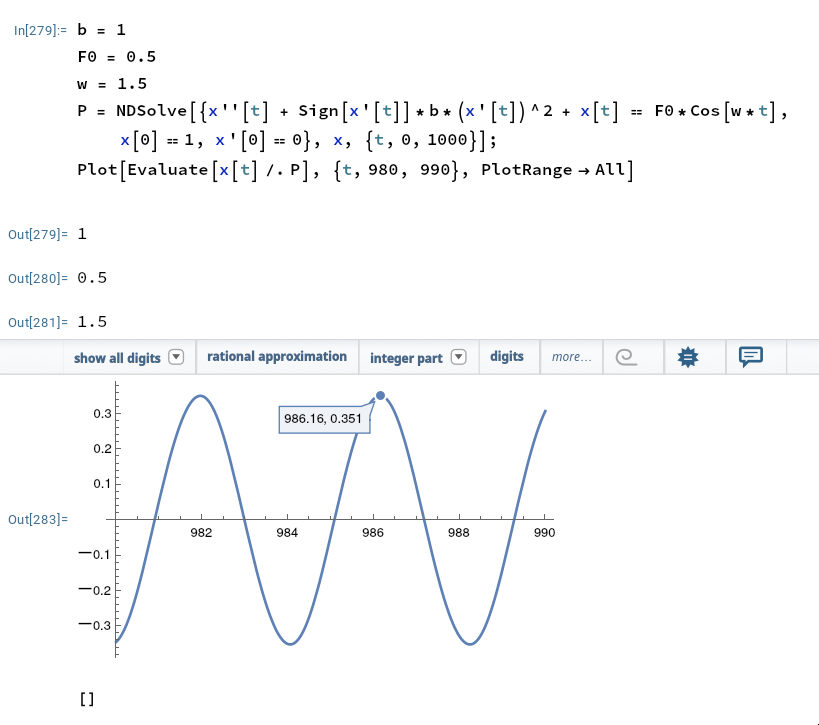
\includegraphics[width=0.8\textwidth]{ss/sshw4/tg1.png}
	\caption{I take the reading by manually by changing the values one by one and individually reading peaks at some time $t \gg 1$}
	\label{fig:ss-sshw4-tg1-png}
\end{figure}
\begin{figure}[H]
	\centering
	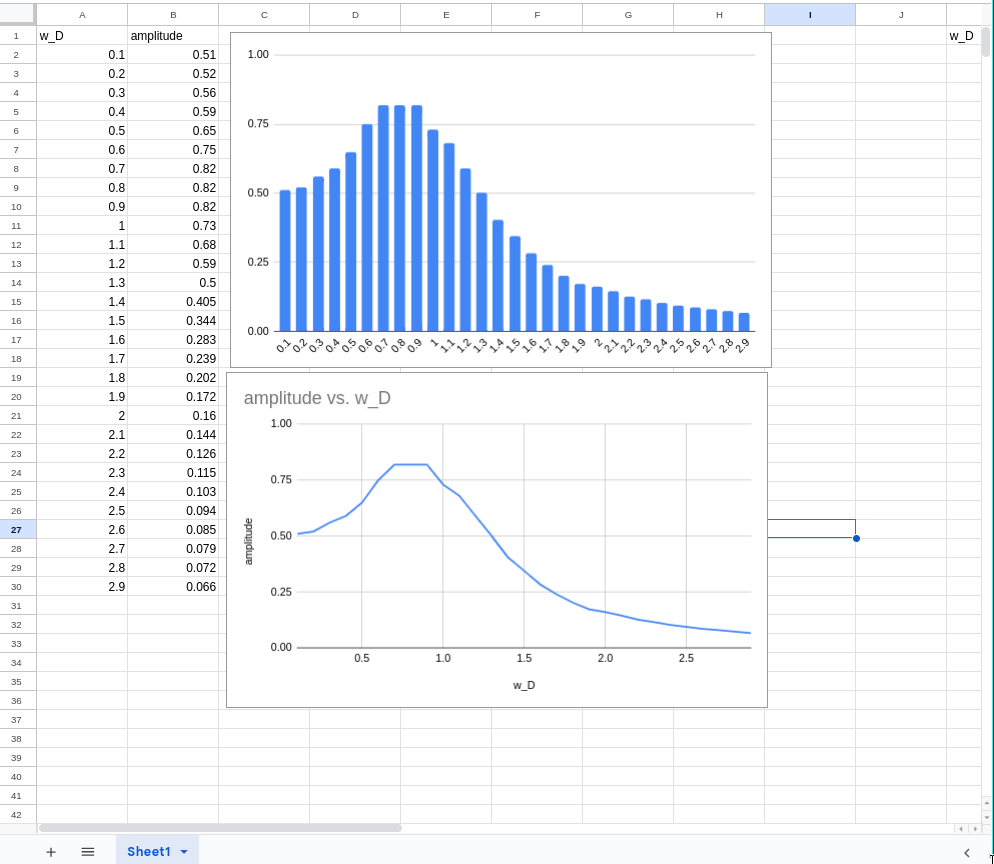
\includegraphics[width=0.8\textwidth]{ss/sshw4/tg2.png}
	\caption{Non linear dampening where $A$ is plotted against $\omega_D$}
	\label{fig:ss-sshw4-tg2-png}
\end{figure}
\newpage
I repeat the tedious process for linear case 
\[
\ddot{x} +(1) (\dot{x})  + \omega  = (0.5) \cos(\omega_D t)
\]
\begin{figure}[H]
	\centering
	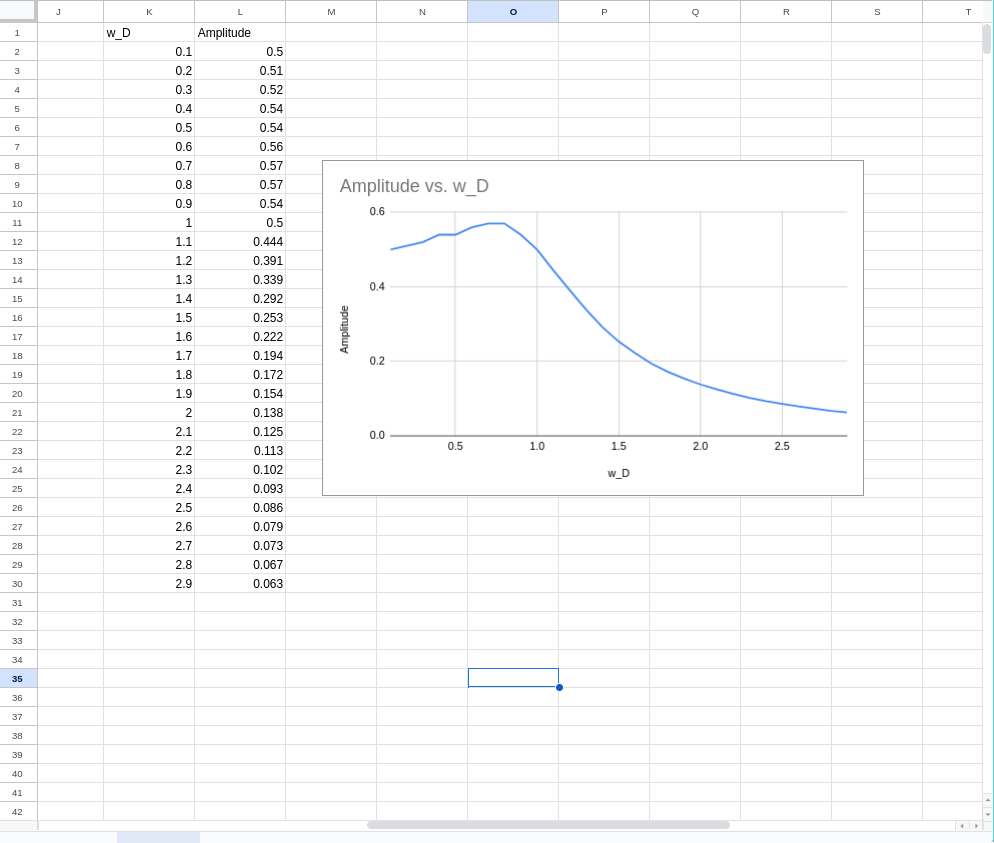
\includegraphics[width=0.8\textwidth]{ss/sshw4/tg3.png}
	\caption{Linear dampening where $A$ is plotted against $\omega_D$}
	\label{fig:ss-sshw4-tg2-png}
\end{figure}



\newpage\section*{WRONG MATHS I DID FOR PROBLEM ONE}
couldn't just erase them because they look good tho 

Consider the real part of this
\begin{align*}
	\frac{C}{- \omega^2 + 2 i \gamma \omega + \omega_0^2 } e^{i \omega t} &=  
	\frac{C}{- \omega^2 + 2 i \gamma \omega + \omega_0^2 } \left(\cos \left(\omega t\right) + i \sin \left(\omega t\right)\right) 
	\\ & \implies \frac{C}{\sqrt{(\omega_0^2 - \omega^2 )^2 + 4\beta^2 \omega^2} } \cos \left(\omega t\right) 
\end{align*}
\subsection*{a} 
External driving force 
\[ F = C e^{i \omega t}
\]
Work done with proper change of coordinates from $\mathrm{d} x$ to $\mathrm{d} t$, we seek the time interval to be a full cycle $ t_i = 2 n \pi / \omega$ to $t_f = 2 (n+1) \pi / \omega$
\begin{align*} 
- W = 
	\int_{x_i}^{x_f}  F \, \mathrm{d} x &=
\int_{t_i}^{t_f}  F(t) \left(\frac{\mathrm{d} x}{\mathrm{d} t}\right) \, \mathrm{d} t \\
&= 
\int_{t_i}^{t_f} (C e^{i \omega t}) \left(\frac{\mathrm{d} }{\mathrm{d} t} 
\left[\frac{C}{- \omega^2 + 2 i \gamma \omega + \omega_0^2} e^{i \omega t}
\right]\right)  \, \mathrm{d} t \\ &=  
\int_{t_i}^{t_f} (C e^{i \omega t}) \left(
\frac{ i \omega C}{- \omega^2 + 2 i \gamma \omega + \omega_0^2} e^{i \omega t}
\right)  \, \mathrm{d} t \\ 
&= 
\int_{t_i}^{t_f} 
\frac{ i \omega C^2 }{- \omega^2 + 2 i \gamma \omega + \omega_0^2} 
e^{2 i \omega t }
\, \mathrm{d} t \\ &=
\frac{ i \omega C^2 }{- \omega^2 + 2 i \gamma \omega + \omega_0^2} 
\left(
\frac{1}{2 i \omega } e^{2 i \omega t}   
\right)\Biggr\rvert_{t_i}^{t_f}  
\\		   &= 
\frac{ C^2 }{ 2 (- \omega^2 + 2 i \gamma \omega + \omega_0^2)} 
\left(
e^{2 i \omega t_f }- e^{ 2 i \omega t_i}   
\right) 
\\		   &= 
\frac{ C^2 }{ 2 (- \omega^2 + 2 i \gamma \omega + \omega_0^2)} 
\left(
	e^{2 i \omega [2(n+1) \pi / \omega }- e^{ 2 i \omega [2 n \pi / \omega ]}   
\right)
		   && \text{ where $n \in \mathbb{Z}^{+}, n \gg 1$}  \\
		   &= 0 
\end{align*} 


\begin{align*}
	-W &= \frac{C^2}{2 A} \left(e^{2 i \omega t_f} - e^{2 i \omega t_i}\right)  \\
\end{align*}

\[
t_i = \frac{2n \pi }{\omega_0} \quad t_f = \frac{2 (n+1) \pi }{\omega_0}
\]
\[
	t_{\frac{1}{2} } = \frac{2 \left(n+ \frac{1}{2}\right) \pi }{\omega_0} = \frac{2n + \pi }{\omega_0} = \frac{2 n }{\omega_0}  + \frac{\pi}{\omega_0}
\]
\[
-W = \frac{C^2}{2A} \left(\cos(2 \omega t_f) + i \sin (2 \omega t_f) - \cos(2 \omega t_i) - i \sin (2 \omega t_i)\right)
\]

\begin{align*}
	-W = \int_{x_i}^{x_f} F \, \mathrm{d} x &= \int_{t_i}^{t_f}   F(t) 
	\left(\frac{\mathrm{d} x}{\mathrm{d} t}\right)\mathrm{d}  t \\
	&= \int_{t_i}^{t_f} (C \cos(\omega t) ) 
	\left( \frac{\mathrm{d} }{\mathrm{d} t} 
		\left[ \frac{C}{- \omega^2 + 2 i \gamma \omega + \omega_0^2 } \cos (\omega t) \right] 
	\right) \mathrm{d} t \\ 
	&= \int_{t_i}^{t_f} (C \cos( \omega t) ) 
	\left(
\frac{ \omega C}{- \omega^2 + 2 i \gamma \omega + \omega_0^2 } (- \sin (\omega t )) 
	\right) \mathrm{d} t\\ 
	&= \frac{- \omega C^2 }{ - \omega^2 + 2 i \gamma \omega + \omega_0^2 } \int_{t_i}^{t_f}  \sin(\omega t) \cos (\omega t ) \mathrm{d}  t \\
	&=  \frac{1}{2 } \frac{- \omega C^2 }{ - \omega^2 + 2 i \gamma \omega + \omega_0^2 } \int_{t_i}^{t_f}  \sin ( 2 \omega t  ) \mathrm{d}  t \\
	&=  \frac{1}{2 } \frac{- \omega C^2 }{ - \omega^2 + 2 i \gamma \omega + \omega_0^2 } 
	\left[ - \cos(2 \omega t) \cdot  \frac{1}{2 \omega} \right]_{t_i}^{t_f}  \\
	&=  \frac{1}{4 } \frac{- C^2 }{ - \omega^2 + 2 i \gamma \omega + \omega_0^2 } 
\left[ - \cos\left(2 \omega \left( \frac{2(n+1)\pi}{\omega} \right)\right) + \cos 
\left(
2 \omega \left( \frac{2 n \pi }{\omega }\right)
\right)\right]  \\ 
	&= 0 
\end{align*}
\textbf{Comment:} This makes sense because the graph of $x(t)$ doesn't go up or down. It stays steady which gives us the sanity check of $W = 0$ for $t \to  \infty$. The driving force does positive work against the drag overshooting the mass, but then does negative work again to balance the overshoot and repeat. This is my intuition for the steady state. 

\subsection*{b}
\begin{align*}
	W &= \int_{x_I}^{x_f} (-F) \, \mathrm{d} x  \\
	  &= \int_{x_i}^{x_f}   \left(2\gamma \frac{\mathrm{d} x}{\mathrm{d} t} \right) \, \mathrm{d} x \\
	  &= \int_{t_i}^{t_f}  2 \gamma \frac{\mathrm{d} x}{\mathrm{d} t} \frac{\mathrm{d} x}{\mathrm{d} t} \, \mathrm{d} t \\ 
	  &=  \int_{t_i}^{t_f} 2 \gamma \left(\frac{\mathrm{d} x}{\mathrm{d} t}\right)^2 \mathrm{d} t \\ &= \int_{t_i}^{t_f}   2 \gamma \left(\frac{ - \omega C}{- \omega ^2 + 2 i \gamma \omega + \omega_0^2  }  \sin(\omega t) \right)^2 \mathrm{d} t\\ 
	  &= 2 \gamma \left(\frac{ - \omega C}{- \omega^2 + 2 i \gamma \omega + \omega_0 ^2 } \right) ^2 \int_{t_i}^{t_f} \sin^2\left( \omega t \right) \, \mathrm{d} t  \\
	  &= 2 \gamma \left(\frac{  - \omega C}{- \omega^2 + 2 i \gamma \omega + \omega_0 ^2 } \right) ^2 
	  \left( \frac{\pi}{ \omega }\right) \\
	  &= \frac{ 2 \pi  \gamma \omega C^2 }{\left(- \omega ^2 + 2 i \gamma \omega + \omega_0^2\right)^2 } \\
\end{align*} 

\[
\frac{1}{2} m v^2(t) = K(t) \implies \Biggr\langle \frac{2 K(t)}{m} \Biggr\rangle = \langle v^2(t) \rangle 
\] 

\[
x(t) = \frac{C}{- \omega^2 + 2 i \gamma \omega + \omega_0^2} \cos(\omega t)
\]

\end{document}
